\documentclass[11pt]{article}
\usepackage{setspace}
\setstretch{1}
\usepackage{amsmath,amssymb, amsthm}
\usepackage{graphicx}
\usepackage{bm}
\usepackage[hang, flushmargin]{footmisc}
\usepackage[colorlinks=true]{hyperref}
\usepackage[nameinlink]{cleveref}
\usepackage{footnotebackref}
\usepackage{url}
\usepackage{listings}
\usepackage[most]{tcolorbox}
\usepackage{inconsolata}
\usepackage[papersize={8.5in,11in}, margin=1in]{geometry}
\usepackage{float}
\usepackage{caption}
\usepackage{esint}
\usepackage{url}
\usepackage{enumitem}
\usepackage{subfig}
\usepackage{wasysym}
\newcommand{\ilc}{\texttt}
\usepackage{etoolbox}
\usepackage{algorithm}
\usepackage{changepage}
% \usepackage{algorithmic}
\usepackage[noend]{algpseudocode}
\usepackage{tikz}
\usetikzlibrary{matrix,positioning,arrows.meta,arrows}
\patchcmd{\thebibliography}{\section*{\refname}}{}{}{}
% \PassOptionsToPackage{hyphens}{url}\usepackage{hyperref}

\providecommand{\myceil}[1]{\left \lceil #1 \right \rceil }
\providecommand{\myfloor}[1]{\left \lfloor #1 \right \rfloor }


\begin{document}



\title{\textbf{CSDS 455: Homework 14}}

\author{Shaochen (Henry) ZHONG, \ilc{sxz517}}
\date{Due and submitted on 10/12/2020 \\ Fall 2020, Dr. Connamacher}
\maketitle


\section*{Problem 1}

\begin{proof}

\leavevmode\newline


    \begin{adjustwidth}{1cm}{}

    \begin{proof}
    \textbf{Lemma: For a graph with $\alpha(G)$ number of independent vertices, we have $\chi(G) \geq \frac{|V(G)|}{\alpha(G)}$}.\newline

    Say we color such graph $G$ with $\chi(G)$ colors and we group vertices according to their color. It is intuitive to tell that $\chi(G)$ will size of the color group with largest cardinality. Since vertices from different color group are not adjacent by definition, we know there will be $\alpha(G)$ color groups under the $\chi(G)$-colored $G$. Thus, it is save to say $|V(G)| \leq \alpha(G) \cdot \chi(G)$ as each color group can have at most $\chi(G)$ vertices and we have at most $\alpha(G)$ color groups. By doing a simple transformation we have $\chi(G) \geq \frac{|V(G)|}{\alpha(G)}$.




    \end{proof}

    \end{adjustwidth}

For the graph in question we have $|V(G)| = 3 \cdot 3 + 2 \cdot 2 = 13$, and we know that $\alpha(G) = 2$ as only two non-adjacent component will be independent from eachother, which implies $\chi(G) \geq \frac{13}{2} = 6.5 \Longrightarrow \chi(G) \geq 7$. The graph is 7-chromatic as demonstrated below (each number represents a color):



\begin{figure}[H]
    \centering
    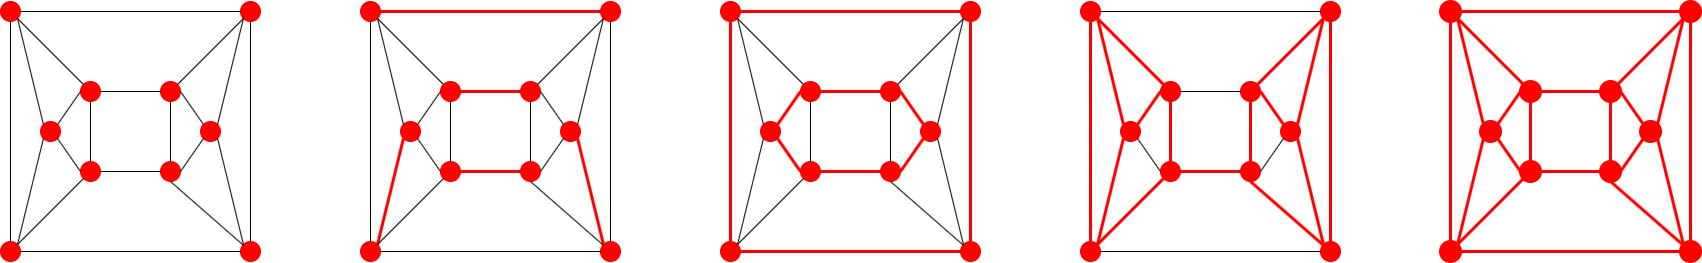
\includegraphics[width=0.4\linewidth]{{fig/fig_p1.png}}
\end{figure}


Now we want to show that this graph does not containa subdivision of 7-clique. Note that each ``component'' of $G$ has either 3 or 2 vertices and we know that a 7-clique has 7 vertices, this suggests that there should be at least two vertices in this 7-clique that are not adjacent to each other, but have 6-vertex-disjoint path between them.\newline

So now we are picking ``2-component'' pairs out of the graph, we have $A$ with $C/D$ (namely a triangle with another triangle), $C/D$ with $B/E$ (a triangle with an edge), or $E$ with $B$.

In the first case, we have 4 vertex-disjoint path from a vertex in $A$ to a vertex in $C/D$ (2 to $B$ and 2 to $E$), $4 < 6$ so this case won't hold up. Similiarily we have 5 vertex-disjoint path in the second case (3 from $D/C$ to $E/B$, 2 internally between $D$ and $C$), $5 < 6$ so the second case won't hold up either.

The third case has 6 vertex-disjoint path (as the edge is adjacent to two triangles). We need 7 of these vertices and we can find them by counting all vertices in ``components''$A, B, E$. Note as we were asked for subdivision of 7-clique, so we will need at least one extra vertex between between the above 7 vertices, however all vertices in $D, C$ (which are the only vertices left to use) do not meed this requirement as regardless which vertex you pick, if it is in $D$ is must go through $C$ and vice versa. Therefore this case eventually also won't hold up. \newline

And as we have showed the graph cannot have a subdivision of a 7-clique, we have completed the prove of the statement.

\end{proof}

\section*{Problem 2}

We first inspect the \textit{lemma} introduced in problem 1. We have $|V(G)| = 3 \cdot 5 = 15$, and we also have $\alpha(G) = 2$ as only two non-adjacent ``components'' will be independent from eachother, which implies $\chi(G) \geq \frac{15}{2} = 7.5 \Longrightarrow \chi(G) \geq 8$. So the graph has the possibility for being 8-chromatic, we have provided one way of doing so below:


\begin{figure}[H]
    \centering
    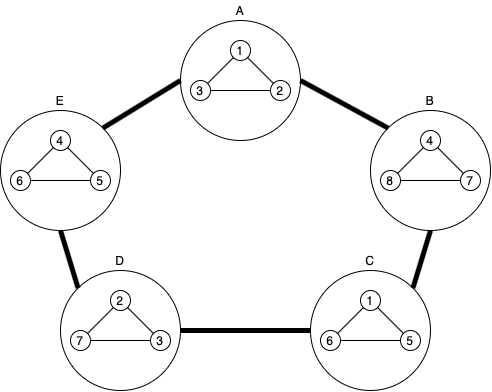
\includegraphics[width=0.4\linewidth]{{fig/fig_p2.png}}
\end{figure}

Now to show this graph does not contain a subdivision of an 8-clique. Knowing that an 8-clique need 8 vertices with 7 vertex-disjoint paths between every two of them, however for any vertex $v$ from the graph, $d(v) = 6$. Therefore we have no subdivision of an 8-clique in this graph.


\section*{Problem 3}

\section*{Problem 4}



% \section{References}
%
% \nocite{*}
% \raggedright
% \bibliography{references.bib}
% \bibliographystyle{plain}


\end{document}